% !TEX root = main_vldb.tex
\label{sec:augmented}
In order to convert the constrained highway dimension to hub labels, we first convert the original graph $G$ (with length and cost functions) into an \emph{augmented graph} $G^B$ with only edge lengths, such that the \emph{efficient paths of $G$ are in bijection with the shortest paths of $G^B$}, i.e. it satisfies
\begin{enumerate}[nosep]
\item All paths starting from a given node are feasible, i.e., they satisfy the budget constraint in $G$.
\item Efficient paths become shortest paths.
\item Inefficient paths are not shortest paths.
\end{enumerate}
We achieve this as follows: Each node in $G^B$ is of the form $\pp{v,b}$, which encodes the information of the remaining budget $b\geq 0$ and location $v\in V$.
A node is connected to neighbors (according to $E$) as long as the remaining budget of that transition is non-negative.
Finally, we create $n$ sink nodes, denoted $v^-$, and connect node $\pp{v,b}$ to $v^-$ with length $1/(b+1)$.
An illustration of the construction is presented in Figure~\ref{fig:augmented}.
Formally, we have
\begin{definition}
Given a network $(G,\ell)$ and $B\in\N$, the augmented version $G^B=(V^B,E^B,\ell^B)$ is defined by
\begin{align*}
V^B &\defeq\crl*{\pp{v,b}: v\in V, b=0,1,\ldots,B}\cup\crl*{v^-:v\in V},\\
E^B &\defeq\crl*{(\pp{v,b},\pp{v',b'}) : vv'\in E, b'=b-c_{vv'}, b'\geq 0}\cup E^{B}_{-},\\
E^{B}_{-} &\defeq \crl*{(\pp{v,b},v^-): v\in V, B\geq b\geq 0}
\end{align*}
and with length function $\ell^B(\cdot)$
\begin{align*}
\ell^B(\pp{v,b},v^-) \defeq \frac{1}{b+1}\;,\;
\ell^B(\pp{v,b},\pp{v',b'}) \defeq \ell(vv')
\end{align*}
\end{definition}



\begin{figure}
\label{fig:augmented}
\begin{center}
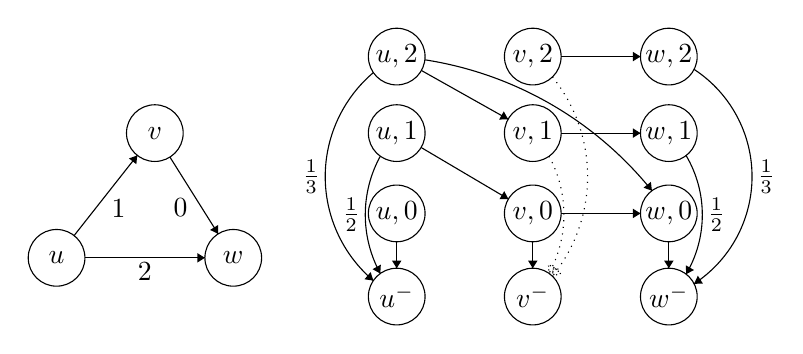
\begin{tikzpicture}[scale=0.12]
\tikzstyle{every node}+=[inner sep=0pt]
\draw [black] (5,-34.3) circle (3);
\draw (5,-34.3) node {$u$};
\draw [black] (15.4,-21.1) circle (3);
\draw (15.4,-21.1) node {$v$};
\draw [black] (23.7,-34.3) circle (3);
\draw (23.7,-34.3) node {$w$};
\draw [black] (41,-13) circle (3);
\draw (41,-13) node {$u,2$};
\draw [black] (41,-21.1) circle (3);
\draw (41,-21.1) node {$u,1$};
\draw [black] (41,-29.6) circle (3);
\draw (41,-29.6) node {$u,0$};
\draw [black] (41,-38.4) circle (3);
\draw (41,-38.4) node {$u^-$};
\draw [black] (55.4,-13) circle (3);
\draw (55.4,-13) node {$v,2$};
\draw [black] (55.4,-21.1) circle (3);
\draw (55.4,-21.1) node {$v,1$};
\draw [black] (55.4,-29.6) circle (3);
\draw (55.4,-29.6) node {$v,0$};
\draw [black] (55.4,-38.4) circle (3);
\draw (55.4,-38.4) node {$v^-$};
\draw [black] (69.8,-13) circle (3);
\draw (69.8,-13) node {$w,2$};
\draw [black] (69.8,-21.1) circle (3);
\draw (69.8,-21.1) node {$w,1$};
\draw [black] (69.8,-29.6) circle (3);
\draw (69.8,-29.6) node {$w,0$};
\draw [black] (69.8,-38.4) circle (3);
\draw (69.8,-38.4) node {$w^-$};
\draw [black] (6.86,-31.94) -- (13.54,-23.46);
\fill [black] (13.54,-23.46) -- (12.66,-23.78) -- (13.44,-24.39);
\draw (10.77,-29.12) node [right] {$1$};
\draw [black] (17,-23.64) -- (22.1,-31.76);
\fill [black] (22.1,-31.76) -- (22.1,-30.82) -- (21.25,-31.35);
\draw (18.92,-29) node [left] {$0$};
\draw [black] (8,-34.3) -- (20.7,-34.3);
\fill [black] (20.7,-34.3) -- (19.9,-33.8) -- (19.9,-34.8);
\draw (14.35,-34.8) node [below] {$2$};
\draw [black] (43.98,-13.342) arc (81.20715:38.87551:38.409);
\fill [black] (68.01,-27.19) -- (67.9,-26.26) -- (67.12,-26.88);
\draw [black] (43.58,-22.62) -- (52.82,-28.08);
\fill [black] (52.82,-28.08) -- (52.38,-27.24) -- (51.87,-28.1);
\draw [black] (58.4,-29.6) -- (66.8,-29.6);
\fill [black] (66.8,-29.6) -- (66,-29.1) -- (66,-30.1);
\draw [black] (43.61,-14.47) -- (52.79,-19.63);
\fill [black] (52.79,-19.63) -- (52.33,-18.8) -- (51.84,-19.67);
\draw [black] (58.4,-21.1) -- (66.8,-21.1);
\fill [black] (66.8,-21.1) -- (66,-20.6) -- (66,-21.6);
\draw [black] (58.4,-13) -- (66.8,-13);
\fill [black] (66.8,-13) -- (66,-12.5) -- (66,-13.5);
\draw [black] (72.471,-14.353) arc (56.79859:-56.79859:13.561);
\fill [black] (72.47,-37.05) -- (73.41,-37.03) -- (72.87,-36.19);
\draw (79.11,-25.7) node [right] {$\frac{1}{3}$};
\draw [black] (71.625,-23.471) arc (30.61438:-30.61438:12.329);
\fill [black] (71.63,-36.03) -- (72.46,-35.59) -- (71.6,-35.09);
\draw (73.84,-29.75) node [right] {$\frac{1}{2}$};
\draw [black] (69.8,-32.6) -- (69.8,-35.4);
\fill [black] (69.8,-35.4) -- (70.3,-34.6) -- (69.3,-34.6);
\draw [black] (38.528,-36.71) arc (-130.31667:-229.68333:14.439);
\fill [black] (38.53,-36.71) -- (38.24,-35.81) -- (37.59,-36.57);
\draw (32.93,-25.7) node [left] {$\frac{1}{3}$};
\draw [black] (39.265,-35.961) arc (-151.22419:-208.77581:12.903);
\fill [black] (39.26,-35.96) -- (39.32,-35.02) -- (38.44,-35.5);
\draw (37.17,-29.75) node [left] {$\frac{1}{2}$};
\draw [black] (41,-32.6) -- (41,-35.4);
\fill [black] (41,-35.4) -- (41.5,-34.6) -- (40.5,-34.6);
\draw [black] (55.4,-32.6) -- (55.4,-35.4);
\fill [black] (55.4,-35.4) -- (55.9,-34.6) -- (54.9,-34.6);
\draw [dotted] (57.481,-15.155) arc (38.87983:-38.87983:16.799);
\draw [densely dotted] (57.48,-36.24) -- (58.37,-35.94) -- (57.59,-35.31) -- cycle;
\draw [dotted] (57.121,-23.549) arc (28.47781:-28.47781:13.004);
\draw [densely dotted] (57.12,-35.95) -- (57.94,-35.49) -- (57.06,-35.01) -- cycle;
\end{tikzpicture}
\end{center}
\caption{Example of a graph augmentation: The original graph $G$ has all paths of unit length, and costs as labeled on the edges. In the augmented graph $G^B$, the labels represent the edge lengths (unlabeled edges have length 1). Note the additional edges from $(w,B)$ to the sink node $w^-$ (the corresponding links to the sinks $u^-,v^-$ have not been shown for exposition purposes). 
}
\end{figure}


Paths in $G^B$ are mapped to paths in $G$ in the intuitive way, by removing the budget labels and sink nodes. Formally
\begin{definition}
Let $P$ be a path in $G^B$.
If $P$ is of the form $\prn*{\pp{v_1,b_1},\ldots,\pp{v_k,b_k}}$, then the projection of $P$, denoted $\bar P$, is the path $\bar P\defeq v_1v_2\ldots v_k$.
Analogously, if $P$ is of the form $\prn*{\pp{v_1,b_1}\ldots\pp{v_k,b_k}v_{k}^-}$, then $\bar P\defeq v_1\ldots v_{k}$. 
\end{definition}


\begin{proposition}\label{prop:shorteffic}
A shortest path from source $\pp{s,b}$ to sink node~$t^-$ projects to an efficient path in $G$ solving $\dist(s,t|b)$. 
\end{proposition}
\begin{proof}
Let $P$ be the shortest path from $\pp{s,b}$ to $t^-$, and $\bar P$ its projection.
To reach $t^-$, $P$ must pass through some $\pp{t,b'}$, $b'\geq 0$.
By construction, $P$ consumes $b-b'$ units of resource, hence it is feasible; moreover, $\bar P$ is the shortest among $(s,t)$-paths with cost $b-b'$.
Now assume, by way of contradiction, that $\bar P$ is not efficient.
As $\bar P$ is the shortest using $b-b'$ units of resource, there exists $P'$ such that $\ell(\bar P')\leq \ell(\bar P)$ and $c(\bar P')< c(\bar P)$.
It must be that $P'$ passes through $\pp{t,b''}$, with $b''>b'$.
We argue that, in this case, $P$ would not be a shortest path to $t^-$.
Indeed, 
\[
\ell(P')=\ell(\bar P')+\frac{1}{1+b''}
\leq \ell(\bar P) +\frac{1}{1+b''}
< \ell(\bar P) +\frac{1}{1+b'},
\]
where the last expression is exactly $\ell(P)$.
\end{proof}

We note that the augmented graph is similar to existing techniques for solving CSP via dynamic programming~\cite{alex_bicriteria}; such an approach however requires that all costs are non-zero (and thus the augmented graph is a DAG).
In contrast, we allow edge costs to be zero, and therefore, our augmented graph may contain cycles. 

The above result now allows us to relate EPHS of the original graph to LSHS in the augmented graph.
Note that in $G^B$, we are interested only in shortest paths ending in sink nodes (since these project to efficient paths). 
Let $\calP^B$ be the path-system comprising all shortest paths in $G^B$ ending in a sink node.
A hitting set for $\PE$ can be used to obtain a hitting set for $\calP^B$, but, since the augmented graph has more nodes, the sparsity increases.
 
\begin{proposition}
If the path-system $\PE$ admits $(\hc,r)$-EPHS, then $\calP^B$ admits $(\hc B,r)$-LSHS.
\end{proposition}
\begin{proof}
%We define a set $C^B$ and prove that hits $\calP_r^B$ and that it is locally sparse.
Given $C$, an $(\hc,r)$-EPHS for $\PE$, define
\begin{equation}\label{eq:hitset}
C^B\defeq \{\pp{v,b}: v\in C, v \text{ hits }\bar P\in\calP_r^B, c(\bar P)=b\leq B \}.
\end{equation}

By Proposition~\ref{prop:shorteffic}, we know that shortest paths are efficient, hence $C^B$ hits all the desired paths.
Finally, we prove local sparsity.
Take any node $\pp{u,b}$ and observe that
\begin{align*}
\Bf_{2r}(\pp{u,b}) &= \{\pp{v,x}: \exists P\in\calP_{u,v}, \ell(P)\leq 2r, c(P)=b-x\} \\
&\subseteq \{\pp{v,x}: v\in \Bf_{2r}(u), x\leq b\} .
\end{align*}
We know that $\card{\Bf_{2r}(u)\cap C}\leq \hc$, therefore $\card{\Bf_{2r}(\pp{u,b})\cap C^B}\leq\hc b\leq \hc B$.
A similar argument shows the sparsity for the reverse ball.
\end{proof}

%\begin{remark}
The proof above shows a stronger result:
In Equation~(\eqref{eq:hitset}) we see that the sparsity around the node $\pp{u,b}$ is $\hc b$.
This is key for our subsequent query time guarantees.
%\end{remark}
%The last result shows how LSHS translate to the augmented graph.
%Since the notion of HD is stronger, it is not always possible to make the analogous between two path systems. Surprisingly, in this case we are able to relate the HD of both path systems.
Moreover, we can also relate the highway dimensions of the path-systems $\PE$ and $\calP^B$ (Note: this does not follow from above, since the HD is a stronger notion than existence of locally-sparse hitting sets).
\begin{proposition}\label{prop:HDaugmented}
If the HD of the system $\PE$ is $h_c$, then the HD of the system $\calP^B$ is $Bh_c$.
\end{proposition}
\begin{proof}
Fix $r>0$ and $\pp{v,b}\in V^B$ .
Let $H_{v,r}\subseteq V$ be the set hitting $S_r(v,\PE)$ and define $H\defeq H_{v,r}\times\{0,1,\ldots,B\}$.
We show that $H$ hits $\Sf_r(\pp{v,b},\calP^B)$.

Take $P\in\Sf_r(\pp{v,b},\calP^B)$.
Since $\dist(\pp{v,b},P)\leq 2r$, it holds $\dist(v,\bar P)\leq 2r$, therefore $\bar P\in \Sf_r(v,\PE)$.
Finally, $H_{v,r}$ hits $\bar P$, thus $H$ hits $P$.
A similar argument shows that $H$ hits $\Sb_r(\pp{v,b},\calP^B)$.
\end{proof}

\sbedit{
It is interesting that, assuming doubling dimension $\alpha$ and $\beta$-witness, we obtain sparsity of $\alpha^{\beta} hB$ and thus query times of $O(\alpha^{\beta} hB\log D)$ \anote{now the witness is defined later}. This is much better than the $O(Bn\Delta)$ of dynamic programming, but it is still pseudo-polynomial. We observe that the query time can be made strongly polynomial if and only if the Pareto frontier contains at most a poly-logarithmic number of points. See Section~\ref{sec:frontier} for a further discussion on this.


Pointer to practical augmented graph.}
